% Created 2022-03-09 Wed 15:12
% Intended LaTeX compiler: pdflatex
\documentclass[11pt]{article}
\usepackage[utf8]{inputenc}
\usepackage[T1]{fontenc}
\usepackage{graphicx}
\usepackage{longtable}
\usepackage{wrapfig}
\usepackage{rotating}
\usepackage[normalem]{ulem}
\usepackage{amsmath}
\usepackage{amssymb}
\usepackage{capt-of}
\usepackage{hyperref}
\input{../../../../preamble-lite.tex}
\author{Qi'ao Chen\\21210160025}
\date{\today}
\title{2}
\hypersetup{
 pdfauthor={Qi'ao Chen\\21210160025},
 pdftitle={2},
 pdfkeywords={},
 pdfsubject={},
 pdfcreator={Emacs 28.0.90 (Org mode 9.6)}, 
 pdflang={English}}
\begin{document}

\maketitle
\begin{exercise}
\((\C,+,\cdot)\) is an algebraically closed field. Show that the algebraic set \(\{(x,y)\in\C^2:x^2+y^2=0\}\)
  is reducible, i.e., not a variety
\end{exercise}

\begin{proof}
Since \(x^2+y^2=(x+yi)(x-yi)\), \(\{(x,y)\in\C^2:x^2+y^2=0\}=\{(x,y)\in\C^2:x+yi=0\}\cup\{(x,y)\in\C^2:x-yi=0\}\)
\end{proof}

\begin{exercise}
Consider the theory of dense linear orders. Let \(\varphi(x,y)\) be the formula \(x<y\). One can show
that \(\varphi(x,y)\) has dichotomy property. Show by giving an example that \(D_3\) is consistent
\end{exercise}

\begin{proof}
Consider
\begin{center}\begin{tikzpicture}
\Tree [.\(y:0\)  [.\(y_0:-4\) [.\(y_{00}:-6\) \(x_{000}:-7\) \(x_{001}:-5\) ]
                                               [.\(y_{01}:-2\) \(x_{010}:-3\) \(x_{011}:-1\) ] ]
                            [.\(y_1:4\) [.\(y_{10}:2\) \(x_{100}:1\) \(x_{101}:3\) ]
                                           [.\(y_{11}:6\) \(x_{110}:5\) \(x_{111}:7\) ] ] ]
\end{tikzpicture}\end{center}
\end{proof}

\begin{exercise}
In the structure \(M=(\R,+,\cdot,0,1,\le)\), let \(\varphi(\barx,\bary)\) be the formula \(x_1y_1+x_2y_2=1\).
Thus \(\varphi(\R^2,\barb)\) is a line for most \(\barb\in\R^2\). It turns out that the formula \(\varphi\) does not have
the dichotomy property. Find the largest \(n\) s.t. \(D_n\) is consistent
\end{exercise}

\begin{proof}
Largest \(n\) is 1. For a fixed \(\bary=(a,b)\) with \(ab\neq 0\), we could take \(\barx_0\) on the
line of \(xy=1-ab\) and \(\barx_0\) outside the line.

Now for \(n=2\), suppose we
have \(\bary=(a,b)\), \(\bary_0=(a_0,b_0)\), \(\bary_1=(a_1,b_1)\), \(\barx_{ij}=(a_{ij},b_{ij})\)
for \(i,j=0,1\) and \(D_n\) is consistent. Then
since \(\varphi(\barx_{00},\bary)\) and \(\varphi(\barx_{01},\bary)\).

Suppose \(ab=1\), then \(a_{00}b_{00}=a_{01}b_{01}=0\).
Since \(\varphi(\barx_{00},\bary_0)\), \(a_0b_0=1\) and hence \(\varphi(\barx_{01},\bary_1)\), a contradiction.

Now since \(ab\neq 1\), \(\barx_{00}\) and \(\barx_{01}\) are on the same line \(xy=1-ab\), and there
is no such \(\bary_0\) to get a line \(xy=1-a_0b_0\) to isolate \(\barx_{00}\) and \(\barx_{01}\).

Thus \(D_2\) is inconsistent
\end{proof}

\begin{exercise}
Let \(T\) be a complete theory of the structure \((\Z,+,-,0)\). Show that \(T\) is not \(\aleph_0\)-stable
\end{exercise}

\begin{proof}
Suppose we are working in base-2 system.

Given \(\sigma\in 2^{<\omega}\), let \(\phi_{\sigma 0}(x)=\exists y(x=y\cdot(10)^{\lh(\sigma)+2}+\sigma)\)
and \(\phi_{\sigma 1}(x)=\exists(x=y\cdot(10)^{\lh(\sigma)+2}+\sigma+1\cdot(10)^{\lh(\sigma)+1})\) where \(\lh(\sigma)\) denotes the length of
\(\sigma\). Then \(\phi_{\sigma i}(x)\Leftrightarrow\) \(x\) extends \(\sigma i\) for \(i=0,1\). Thus we have a tree
\begin{center}\begin{tikzpicture}
\Tree [.\(\phi\)  [.\(\phi_0\) [.\(\phi_{00}\) \(\vdots\) \(\vdots\) ]
                                               [.\(\phi_{01}\) \(\vdots\) \(\vdots\) ] ]
                            [.\(\phi_1\) [.\(\phi_{10}\) \(\vdots\) \(\vdots\) ]
                                           [.\(\phi_{11}\) \(\vdots\) \(\vdots\) ] ] ]
\end{tikzpicture}\end{center}
where \(\phi\) is \(x=x\).

Now note that for any \(\sigma\in 2^{<\omega}\) \(\phi_{\sigma}\leftrightarrow\phi_{\sigma 0}\vee\phi_{\sigma 1}\) and \(\phi_{\sigma i}\vDash\neg\phi_{\sigma(1-i)}\)
for \(i=0,1\). For each \(f:\omega\to 2\), \([\phi_{f\mid 1}]\supseteq[\phi_{f\mid 2}]\supseteq\cdots\) and since \(S_1(\Z)\) is compact,
there is \(p_f\in\bigcap_{i\in\omega}[\phi_{f\mid i}]\). If \(f,g\in 2^\omega\) and \(f\neq g\), then there is \(n\)
s.t. \(f(n)\neq g(n)\) and \(f\mid n=g\mid n\). Then
since \(\phi_{f\mid(n+1)}\vDash\neg\phi_{g\mid (n+1)}\), \([\phi_{f\mid n+1}]\cap[\phi_{g\mid n+1}]=\emptyset\) and hence \(p_f\neq p_g\).
Thus \(\abs{S_1(\Z)}\ge 2^{\aleph_0}\)
\end{proof}
\end{document}
